
%%%%%%%%%%%%%%%%%%%%%%%%%%%%%%%%%%%%%%%%%%%%%%%%%%%%%%%%%%%%%%%%%%%%%
%% This is a (brief) model paper using the achemso class
%% The document class accepts keyval options, which should include
%% the target journal and optionally the manuscript type.
%%%%%%%%%%%%%%%%%%%%%%%%%%%%%%%%%%%%%%%%%%%%%%%%%%%%%%%%%%%%%%%%%%%%%
\documentclass[journal=apchd5,manuscript=article]{achemso}

%%%%%%%%%%%%%%%%%%%%%%%%%%%%%%%%%%%%%%%%%%%%%%%%%%%%%%%%%%%%%%%%%%%%%
%% Place any additional packages needed here.  Only include packages
%% which are essential, to avoid problems later. Do NOT use any
%% packages which require e-TeX (for example etoolbox): the e-TeX
%% extensions are not currently available on the ACS conversion
%% servers.
%%%%%%%%%%%%%%%%%%%%%%%%%%%%%%%%%%%%%%%%%%%%%%%%%%%%%%%%%%%%%%%%%%%%%
\usepackage[version=3]{mhchem} % Formula subscripts using \ce{}
\usepackage[T1]{fontenc}       % Use modern font encodings
\usepackage{graphicx}
\usepackage{amsmath}
\usepackage{xcolor}
\usepackage{wrapfig}
%\usepackage{multline}
%%%%%%%%%%%%%%%%%%%%%%%%%%%%%%%%%%%%%%%%%%%%%%%%%%%%%%%%%%%%%%%%%%%%%
%% If issues arise when submitting your manuscript, you may want to
%% un-comment the next line.  This provides information on the
%% version of every file you have used.
%%%%%%%%%%%%%%%%%%%%%%%%%%%%%%%%%%%%%%%%%%%%%%%%%%%%%%%%%%%%%%%%%%%%%
%%\listfiles

%%%%%%%%%%%%%%%%%%%%%%%%%%%%%%%%%%%%%%%%%%%%%%%%%%%%%%%%%%%%%%%%%%%%%
%% Place any additional macros here.  Please use \newcommand* where
%% possible, and avoid layout-changing macros (which are not used
%% when typesetting).
%%%%%%%%%%%%%%%%%%%%%%%%%%%%%%%%%%%%%%%%%%%%%%%%%%%%%%%%%%%%%%%%%%%%%
\newcommand*\mycommand[1]{\texttt{\emph{#1}}}

%%%%%%%%%%%%%%%%%%%%%%%%%%%%%%%%%%%%%%%%%%%%%%%%%%%%%%%%%%%%%%%%%%%%%
%% Meta-data block
%% ---------------
%% Each author should be given as a separate \author command.
%%
%% Corresponding authors should have an e-mail given after the author
%% name as an \email command. Phone and fax numbers can be given
%% using \phone and \fax, respectively; this information is optional.
%%
%% The affiliation of authors is given after the authors; each
%% \affiliation command applies to all preceding authors not already
%% assigned an affiliation.
%%
%% The affiliation takes an option argument for the short name.  This
%% will typically be something like "University of Somewhere".
%%
%% The \altaffiliation macro should be used for new address, etc.
%% On the other hand, \alsoaffiliation is used on a per author basis
%% when authors are associated with multiple institutions.
%%%%%%%%%%%%%%%%%%%%%%%%%%%%%%%%%%%%%%%%%%%%%%%%%%%%%%%%%%%%%%%%%%%%%
\author{Nicholas P. Montoni}
\author{Steven C. Quillin}
\author{Charles Cherqui}
\author{David J. Maisello}
\affiliation[Department of Chemistry, University of Washington]
{Department of Chemistry, University of Washington, Seattle, WA 98195}
\email{masiello@chem.washington.edu}
\date{September 4, 2017}
%%%%%%%%%%%%%%%%%%%%%%%%%%%%%%%%%%%%%%%%%%%%%%%%%%%%%%%%%%%%%%%%%%%%%
%% The document title should be given as usual. Some journals require
%% a running title from the author: this should be supplied as an
%% optional argument to \title.
%%%%%%%%%%%%%%%%%%%%%%%%%%%%%%%%%%%%%%%%%%%%%%%%%%%%%%%%%%%%%%%%%%%%%
\title[]
    {Tunable Spectral Ordering and Directional Radiation in Magnetic Plasmon Oligomers}
%%%%%%%%%%%%%%%%%%%%%%%%%%%%%%%%%%%%%%%%%%%%%%%%%%%%%%%%%%%%%%%%%%%%%
%% Some journals require a list of abbreviations or keywords to be
%% supplied. These should be set up here, and will be printed after
%% the title and author information, if needed.
%%%%%%%%%%%%%%%%%%%%%%%%%%%%%%%%%%%%%%%%%%%%%%%%%%%%%%%%%%%%%%%%%%%%%
\abbreviations{MNP, LSPR, EELS}
\keywords{plasmon, hybridization, magnetic, retardation}

%%%%%%%%%%%%%%%%%%%%%%%%%%%%%%%%%%%%%%%%%%%%%%%%%%%%%%%%%%%%%%%%%%%%%
%% The manuscript does not need to include \maketitle, which is
%% executed automatically.
%%%%%%%%%%%%%%%%%%%%%%%%%%%%%%%%%%%%%%%%%%%%%%%%%%%%%%%%%%%%%%%%%%%%%
\begin{document}

%%%%%%%%%%%%%%%%%%%%%%%%%%%%%%%%%%%%%%%%%%%%%%%%%%%%%%%%%%%%%%%%%%%%%
%% The "tocentry" environment can be used to create an entry for the
%% graphical table of contents. It is given here as some journals
%% require that it is printed as part of the abstract page. It will
%% be automatically moved as appropriate.
%%%%%%%%%%%%%%%%%%%%%%%%%%%%%%%%%%%%%%%%%%%%%%%%%%%%%%%%%%%%%%%%%%%%%
\begin{tocentry}
\begin{centering}
\includegraphics[width=7cm]{toc.png}
\end{centering}
\end{tocentry}

%%%%%%%%%%%%%%%%%%%%%%%%%%%%%%%%%%%%%%%%%%%%%%%%%%%%%%%%%%%%%%%%%%%%%
%% The abstract environment will automatically gobble the contents
%% if an abstract is not used by the target journal.
%%%%%%%%%%%%%%%%%%%%%%%%%%%%%%%%%%%%%%%%%%%%%%%%%%%%%%%%%%%%%%%%%%%%%
\begin{abstract}
Using first-principles theory and simulated cathodoluminescence spectroscopy, the optical-frequency magnetic resonances of cyclic aromatic and hexagonally packed metal nanoparticle clusters are explored. A fully retarded coupled dipole model is employed, expanding upon past work in the field, to explore the dependence of the resonant frequencies and spectral ordering of the magnetic resonances on cluster size. It is shown that magnetic resonances change spectral order as metal nanoparticle oligomers change in size, and that these mode switches are observable in full-wave numerical electrodynamics simulations of angle-resolved cathodoluminescence spectra. Electron-beam spectroscopies are uniquely suited to observing this phenomenon, as they provide nanometer spatial and sub-eV spectral resolution and can preferentially excite one magnetic resonance over another. Furthermore, angle-resolved spectroscopies leverage the specific radiation patterns attributed to each magnetic plasmon, clearly differentiating spectral signatures of each individual magnetic plasmon resonance.
\end{abstract}

%%%%%%%%%%%%%%%%%%%%%%%%%%%%%%%%%%%%%%%%%%%%%%%%%%%%%%%%%%%%%%%%%%%%%
%% Start the main part of the manuscript here.
%%%%%%%%%%%%%%%%%%%%%%%%%%%%%%%%%%%%%%%%%%%%%%%%%%%%%%%%%%%%%%%%%%%%%
\section{introduction}
Clusters of metal nanoparticles (MNPs) that exhibit anomalously strong magnetic fields, called plasmon oligomers or plasmon metamolecules, have been of great interest in recent years. These effects, called magnetic plasmon resonances, have been shown to couple to and enhance the magnetic field of light, exhibit a negative index of refraction at certain frequencies, act anti-reflectively, and even hybridize analogously to electric plasmon resonances\cite{Alu2006,Alu2008,Dionne2011,Cherqui2014,Dionne2016,Cherqui2016,Engheta2017}. Much of this work has focused on the single-oligomer regime, studying systems composed of only one ring of nanoparticles using simple models in the quasistatic limit\cite{Nord2006,Dionne2011,Dionne2016,Capolino2017}. Other approaches have involved studying the infinte-oligomer regime, in which the language of solid-state or condensed matter physics is more appropriate\cite{Schatz2003,Weick2013}. Recently, a disconnect between these size regimes and methods has arisen, leading to open questions in how magnetic plasmon resonances behave in the few-oligomer regime; that is, in the intermediate size regime\cite{NordHal2011,NordHal2012,Cherqui2014,Cherqui2016,Engheta2017}.

Most crucial to this concept is the question of when and how retardation effects matter when decribing magnetic plasmon resonances using analytical models. Previous work shows that for a cluster of only two oligomers, the quasistatic approximation breaks down when compared with full-wave simulations in that it predicts a different energy-ordering of magnetic plasmons than in simulated electron energy-loss spectroscopy (EELS) and cathodoluminescence (CL) experiments\cite{Cherqui2014}. Retardation effects have been incorporated into models of single MNPs, dimers, infinite chains, and infinite arrays\cite{Kottman2001,Rechbacher2003,Schatz2003,Royer2005,vonPlessen2007,Abajo2008,Chumanov2010,Gu2010,Pinchuk2016}. However, few studies have shown whether retardation effects are needed to accurately predict the behavior of magnetic plasmon resonances specifically. We aim to show that the incorporation of retardation effects actually corrects the aformentioned discrepancy between models of magnetic plasmon resonances and simulated experiments.

Because retardation effects depend on size and we are interested in the intermediate size regime, we will analyze the energetics of magnetic plasmon resonances as a function of cluster size. At small sizes, magnetic oligomers behave quasistatically; a fully retarded coupled-dipole model and a quasistatic coupled-dipole model make similar predictions, and both models agree with static simulations. However, with increasing size, magnetic oligomers deviate from quasistatic behavior and we predict never-before-reported eigenmode switching of the magnetic plasmon resonances. This is not a theoretical artifact and we demonstrate that, due to magnetic plasmon resonances' distinct radiative properties, this mode switching can be observed in angle-resolved CL spectra using full-wave simulations\cite{Hohenester2012}. Indeed, directional radiation has been previously detected using this technique\cite{Coenen2011,CoPol2011,Polman2014}. The spectral order of the magnetic plasmon resonances depends on aggregate size and mophology, meaning that it is tunable. Tunability of the relative phase of magnetic fields in a single MNP cluster may lead to advances in detection methods, anti-reflective coatings, and information processing\cite{Zia2010trans,Noginova2008trans,Wang:13,Fan2015,Wei2015,Shvets2012,Altug2012bio,Nord2011fano,Zhang2006,NordHal2011,NordHal2012}.

\section{Model Systems and Magnetic Plasmon Resonances}

\begin{figure}
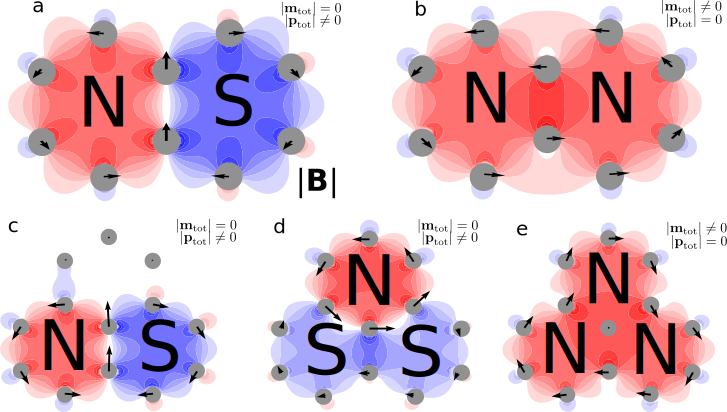
\includegraphics[width=6.5in]{2mer_3mer_fields.pdf}
\caption{Magnetic field plots of the 2mer (a and b) and 3mer (c, d, and e) oligomers. Each system supports a number of closed-loop magnetic plasmon resonances equal to the number of rings in the system. The magnetic plasmons support an electric dipole moment (a, c, and d) support out-of-phase magnetic fields. The nodeless magnetic modes (b and e) support a net magnetic dipole moment are accessible to the magnetic field of light.}
\label{field_plots}
\end{figure}

To begin, we investigate two model systems comprising 10 and 13 silver nanospheres and resembling naphthalene and phenalene, respectively. Diagrams of these systems, from here on called the 2mer and the 3mer, are shown in Figure~\ref{field_plots}. We are interested in the collective eigenmodes of these systems that produce large magentic fields inside the rings and the eigenenergies associated with those modes. Previous work has also attempted to predict the eigenenergies of magnetic oligomer systems, and found that quasistatic predictions of the eigenspectrum, using a coupled dipole method, did not align with simulated EELS of the same oligomers.\cite{Cherqui2014} We modify the previous approach, mapping the individual electric dipole plasmon of each MNP onto a harmonic oscillator and allowing them to couple through retarded dipole-dipole interactions as follows\cite{ARPC}

\begin{equation}
\ddot{\textbf{q}}_i = -\omega_{\textrm{sp}}^2\textbf{q}_i + \frac{e}{m_{\textrm{sp}}}\sum_{j\neq i}\textbf{E}_j(\textbf{r}_i).
\label{equation_of_motion}
\end{equation}

\noindent Here $\omega_{\textrm{sp}}$ is the natural frequency of a single electric plasmon, $m_{\textrm{sp}} = e^2/\alpha_{\textrm{sp}}\omega_{\textrm{sp}}^2$ is the surface plasmon effective mass defined by the polarizability $\alpha_{\textrm{sp}}$, the plasmon oscillator dipole moment $\textbf{d}_i = e\textbf{q}_i$, and $\textbf{E}_j(\textbf{r}_i)$ is the fully retarded electric field from the $j^{\textrm{th}}$ dipole at the position of the $i^{\textrm{th}}$ dipole and is defined as 

\begin{equation}
\textbf{E}_j(\textbf{r}_i) = \boldsymbol{\Lambda}_{ij}\cdot\textbf{d}_j\\
= \left\{\left(\frac{1}{r_{ij}^3} - \frac{ik}{r_{ij}^2}\right)\left(3\hat{\textbf{n}}_{ij}\hat{\textbf{n}}_{ij} - \textbf{1}\right) + \frac{k^2}{r_{ij}}\left(\textbf{1}-\hat{\textbf{n}}_{ij}\hat{\textbf{n}}_{ij}\right)\right\}\frac{e^{\textrm{i}kr_{ij}}}{\varepsilon_b}\cdot\textbf{d}_j.
\label{electric_field_lambda}
\end{equation}

\noindent Here, $\hat{\textbf{n}}_{ij}$ is the unit vector connecting two dipoles separated by distance $r_{ij}$, $k=\sqrt{\varepsilon_b}\omega/c$ is the wavenumber of the collective mode with frequency $\omega$, and $\varepsilon_b$ is the dielectric constant of the background medium. The fully retarded electric field contains three important terms. The term with $1/r_{ij}^3$-dependence is called the near-field, because it decays very quickly with increasing distance. In fact, this term is what remains when taking the quasistatic limit. The second term, with the $k/r_{ij}^2$-dependence, is the intermediate-field term. The third term, with $k^2/r_{ij}$-dependence, is the far-field term, called such because it dominates after the other two have decayed. All three terms are dressed by a complex exponential, which depends both on $k$ and on $r_{ij}$. This shows that at specific separation distances, the interaction energies can change sign and go from energy-lowering to energy-raising. Using just the fully retarded electric field, we have incorporated all necessary retardation effects\cite{Purcell1973}. The full dipole electric field is all that is needed to obtain qualitatively and quantitatively consistent predictions of the behavior of magnetic plasmons. While previous approaches have relied on coarse-graining to build explicit magnetic dipoles into the equations of motion, we show that no such averaging procedure is necessary as the fully retarded electric field contains all of the magnetic information.

Solving the system of Equations~\ref{equation_of_motion} for all of the dipoles in a single aggregate yields as many hybridized modes as there are degrees of freedom, in this case, two times the number of particles. Similarly, each system supports a number of magnetic plasmons equal to the number of oligomers. The eigenvectors of these collective modes represent the dipole moments on each nanoparticle. Figure~\ref{field_plots} shows these magnetic mode eigenvectors overlayed with plots of the signed magnetic field magnitude of each normal mode. Each mode is named for its particular magnetic field distribution after the poles of a magnet, either all-North (aN) or North-South (NS). These magnetic modes have been chosen because each of them can be excited by light and can radiate to the far-field. The top right-hand corner of each field plot in Figure~\ref{field_plots} displays whether the magnetic mode depicted exhibits a net electric dipole or a net magnetic dipole. In planar geometries, the magnetic dipole moments are always perpendicular to the in-plane electric dipole moments. As a result, they scatter light with different directionality. This property will be exploited in angle-resolved spectra to aN magnetic modes from NS magnetic modes.

\section{Spectral Ordering of Magnetic Modes in Model Systems}

To determine the impact of incorporating retardation effects, it is first useful to look at the quasistatic model. Careful observation will show that in the quasistatic limit individual particle frequencies are not dependent on particle size, and the coupling strength is scale-invariant. If the ratio of interparticle distance $r_{ij}$ to particle size $r_0$ remains constant, as the particles grow the collective frequencies should not change. We can see this by rewriting the quasistatic coupling term

\begin{align}
\frac{e^2}{m_{\textrm{sp}}}\boldsymbol{\Lambda}_{ij} &= \frac{e^2}{m_{\textrm{sp}}}\frac{3\hat{\textbf{n}}_{ij}\hat{\textbf{n}}_{ij} - \textbf{1}}{r_{ij}^3} \\
&= \omega_{\textrm{sp}}^2 \alpha_{\textrm{sp}}\frac{3\hat{\textbf{n}}_{ij}\hat{\textbf{n}}_{ij} - \textbf{1}}{r_{ij}^3} \\
&= \omega_{\textrm{sp}}^2 \left(\frac{3r_0^3}{\varepsilon_{\infty}+2}\right)\frac{3\hat{\textbf{n}}_{ij}\hat{\textbf{n}}_{ij} - \textbf{1}}{(sr_0)^3} \\
&= \omega_{\textrm{sp}}^2 \left(\frac{3}{\varepsilon_{\infty}+2}\right)\frac{3\hat{\textbf{n}}_{ij}\hat{\textbf{n}}_{ij} - \textbf{1}}{s^3}.
\label{quasistatic_coupling}
\end{align}

\noindent However, revisiting Equation~\ref{electric_field_lambda} shows that incorporation of retardation effects removes the scale invariance of the coupling by allowing the single plasmon frequency to vary with size and by introducing more size-dependent terms into the coupling (the intermediate- and far-fields). In light of this observation, we choose the scale of the MNP clusters, or the size as a function of an individual MNP radius, as the variable to investigate retardation effects and spectral switching in magnetic plasmon resonances. In all of the explorations, both on the model systems and in future sections, the scale of the system is defined by a nearest-neighbor distance $r_{\textrm{nn}} = 3r_0$, chosen so that each nearest-neighbor pair has a face-to-face separation distance of $r_0$. 

\begin{figure}
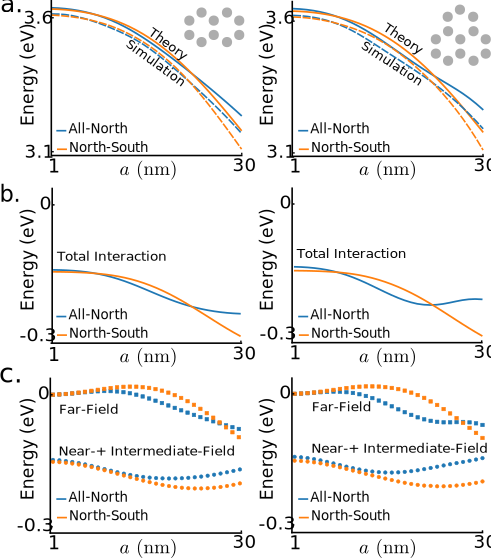
\includegraphics[width=4in]{2mer-3mer-eig.pdf}
\caption{Eigenenergies (a and c) and interaction energies (b and d) for the 2mer and 3mer. At small scales $r_0 < 5$ nm the magnetic modes are ordered as predicted using a quasistatic model, with NS (orange) lower in energy than aN (blue). This implies that for very small oligomer systems, the quasistatic approximation is still accurate. However, at sizes greater than $r_0 = 5$ nm and smaller than $r_0 = 20$ nm, the eigenmodes switch order. This is due to the dominance of the far-field term, which is evident from (b and d). Finally, at sizes greater than $r_0 = 20$ nm, the eigenmodes switch order again. Also plotted are simulated peak positions of each mode (dashed lines) to show agreement within 0.1 eV.}
\label{scaling}
\end{figure}

Figure~\ref{scaling} shows the predicted eigenenergies and the simulated spectral peak positions for the magnetic modes of the 2mer and 3mer with varying $r_0$. At small sizes the magnetic modes preserve the quasistatic ordering predicted in previous work, which is to be expected when the oligomer system fits easily into a wavelength of light and the near-field dominates the electric field\cite{Cherqui2014}. In fact, a fully retarded scattering spectrum of an aggregate of this size is qualitatively identical to quasistatic simulations of the same system at all sizes. This implies that the quasistatic approximation is accurate only for magnetic oligomers spanning less than a quarter of the wavelength of light, smaller than suggested by previous work for single particles [\textbf{I can't find the review paper where they report the $\lambda/2$ number.}]. As the system scale increases, the eigenenergies decrease and appear to cross at $r_0 = 7$ nm, and once more at $r_0 = 20$ nm. This is due to the far-field term in Equation~\ref{electric_field_lambda} becoming strong relative to the near- and intermediate-fields, as shown in Figure~\ref{scaling}b and d (squares). As the system gets larger, it takes information longer to propagate across the aggregate, meaning that retaradtion effects become important. The second crossing of the eigenmodes recovers the ordering at small sizes, which might lead to the erroneaous conclusion that the quasistatic approximation is accurate again. Rather, both eigenmode crossings are due entirely to retardation effects. The interaction energy between all the dipoles in each magnetic mode,

\begin{equation}
U_{\textrm{int}} = -\sum_i \textbf{d}_i \cdot \sum_{j \neq i} \textbf{E}_j(\textbf{r}_i),
\label{interactionenergy}
\end{equation}

\noindent with the same $\textbf{E}_j$ defined in Equation~\ref{electric_field_lambda}, explains why the modes cross at certain system sizes. The inclusion of the far-field, the third term in Equation~\ref{electric_field_lambda} is the cause of the mode switching, as it carries the opposite sign of the near- and intermediate-field terms. These terms with opposite splitting are the cause of the mode crossings; as the near- and intermediate-fields lower the energy of the North-South mode, the far-field raises the energy of the North-South mode, and vice-versa for the North-North mode. Close inspection of Figure~\ref{scaling}b reveals that the crossing points occur where the splitting in the near- and intermediate-fields is equal and opposite to that of the far-field. Perhaps more interestingly, in water the crossing points are shifted towards smaller scale. This is to be expected, as the wavelength of light is compressed in a medium, meaning that light sees objects as much bigger than they really are. This analysis shows that the quasistatic approximation is good for very small magnetic oligomers in vacuum, and for smaller oligomers in medium. This can also be explained through the impact of a dielectric medium on coupling strength. While a medium should contribute an overall increase to the coupling strength (which is predicted in Figure~\ref{scaling}b and f), the far-field term should be more drastically impacted due to its extra $\varepsilon_b$-dependence through its $k^2$ term.\cite{Elsayed2008} Through comparison with simulation (dashed lines in Figure~\ref{scaling}a), it can be shown that this simple and efficient model is accurate to within 0.05 eV and accurately describes the behavior of magnetic plasmon oligomers.

Previous work has explored the oscillatory nature of resonance frequency and radiation damping as a function of size in plasmonic systems\cite{vonPlessen2007}. We have shown that a fully retarded coupled dipole approach predicts magnetic plasmon resonance switching, and explains that it is due to inclusion of the far-field term in the dipole relay tensor. From here, we use simulated angle-resolved CL spectroscopy to observe this magnetic mode switching, leveraging the specific radiative properties of each magnetic plasmon and the ability of the electron beam to isolate specific plasmon modes.

\section{Radiative Properties of Magnetic Plasmon Resonances}
In order to detect the spectral switching of magnetic plasmons, we must exploit their unique radiative properties. Only those magnetic eigenmodes supporting net dipole moments should radiate to the far field. Furthermore, the aN magnetic mode dipole moment is perpendicular to the NS mode electric dipole moment(s) in both the model 2mer and 3mer, meaning that they radiate with different directional-dependence. It has been predicted and shown experimentally that single magnetic oligomers scatter light anisotropically when both their magnetic dipole moment and electric dipole moment are mutually excited.\cite{Dionne2011,Cherqui2016} This is evident from the difference between forward and backward scattering spectra, but can also be shown by computing the differential scattering pattern,\cite{jackson_classical_1999,schwinger1998classical}

\begin{equation}
\frac{dP}{d\Omega} = \frac{c}{8\pi}\textrm{Re}\left[r^2\hat{\textbf{n}}\cdot\sum_i\textbf{E}_i \times \sum_{j}\textbf{B}_{j}^*\right]
\label{dp_field_1}
\end{equation}

\noindent where $\hat{\textbf{n}}$ is the unit vector pointing to the detector a distance $r >> \lambda$ away and $\textbf{E}_i$ and $\textbf{B}_j^*$ are the electric field and conjugate magnetic inductance originating from each oligomer ring. In order to predict the qualitative properties of independently and mutually exciting an orthogonal magnetic and electric plasmon, we coarse-grain our approach by assuming that each ring of the oligomer supports one collective electric and one collective magnetic dipole moment, co-located at the center of each ring. Using the far-fields scattered by such an arrangement of electric and magnetic dipoles reduces the differential scattering to\cite{Engheta2006}

\begin{equation}
\frac{dP}{d\Omega} = \frac{ck_e^2k_m^2}{8\pi} \textrm{Re} \left[\hat{\textbf{n}} \cdot \sum_{i} (\hat{\textbf{n}} \times \textbf{d}_i) \times \hat{\textbf{n}} - \hat{\textbf{n}} \times \boldsymbol{\mu}_i \times \sum_{j} \hat{\textbf{n}} \times \textbf{d}_j^* + (\hat{\textbf{n}} \times \boldsymbol{\mu}_j^*) \times \hat{\textbf{n}}\right]
\label{dp_coarse_grain}
\end{equation}

Performing the vector operations in Equation~\ref{dp_coarse_grain} yields

\begin{multline}
\frac{dP}{d\Omega} = \frac{ck^4}{8\pi} \textrm{Re} [ \sum_{ij} \textbf{d}_i \cdot \textbf{d}_j^* - (\hat{\textbf{n}} \cdot \textbf{d}_i)(\hat{\textbf{n}} \cdot \textbf{d}_j^*) + \boldsymbol{\mu}_i \cdot \boldsymbol{\mu}_j^* - (\hat{\textbf{n}} \cdot \boldsymbol{\mu}_i)(\hat{\textbf{n}} \cdot \boldsymbol{\mu}_j^*) \\ + \hat{\textbf{n}} \cdot (\textbf{d}_i \times \boldsymbol{\mu}_j^* + \textbf{d}_j^* \times \boldsymbol{\mu}_i) ].
\label{dp_dipoles_1}
\end{multline}

\noindent To build intuition, we demand the magnetic dipole $\boldsymbol{\mu}$ is oriented in the z-direction, and the electric dipole $\textbf{d}$ is oriented in the y-direction. The coarse-grained electric dipole and magnetic dipole can be written in terms of their constituent dipoles $\textbf{d} = \sum_n d_{e,n} \hat{\textbf{y}}$ and $\boldsymbol{\mu} = \frac{k_m}{2}\sum_n(\textbf{r}_n \times d_{m,n} \hat{\boldsymbol{\phi}}_n) = \frac{k_mNRd_m}{2}\hat{\textbf{z}}$ where the sums are taken over the $n$-th and $m$-th dipoles, respectively. Using these definitions, reducing the sum to a single oligomer for simplicity, and giving each dipole equivalent magnitude, the differential scattering becomes

\begin{equation}
\frac{dP}{d\Omega} = \frac{N^2ck_e^2k_m^2}{8\pi}\left[ d_e^2(1 - (\hat{\textbf{n}} \cdot \hat{\textbf{y}})^2) + \frac{k_m^2R^2d_m^2}{4}(1 - (\hat{\textbf{n}} \cdot \hat{\textbf{z}})^2) + d_ed_mk_mR(\hat{\textbf{n}} \cdot \hat{\textbf{x}})\right]
\label{dp_dipoles_2}
\end{equation}

Equation~\ref{dp_dipoles_2} shows that exciting different combinations of dipoles leads to very specific radiation patterns. Exciting only a net electric dipole moment and setting $d_m = 0$ results in a dipolar radiation pattern with a node of zero radiation along the electric dipole axi, in this case the y-axis. Similarly, setting $d_e = 0$ and exciting only a net magnetic dipole results in another dipolar radiation pattern with a node along the magnetic dipole axis, which in this case is the z-axis. Finally, exciting both an electric and a magnetic dipole results in contributions from both patterns in the y- and z-directions. However, the third term of Equation~\ref{dp_dipoles_2} contributes an asymmetry, increasing the radiation in the positive x-direction, or the forward direction in this case, while decreasing the radiation in the backwards direction. This intuitively shows that interfering othrogonal electric and magnetic plasmons radiate with low or no back scattering\cite{Dionne2011}.

\begin{figure}
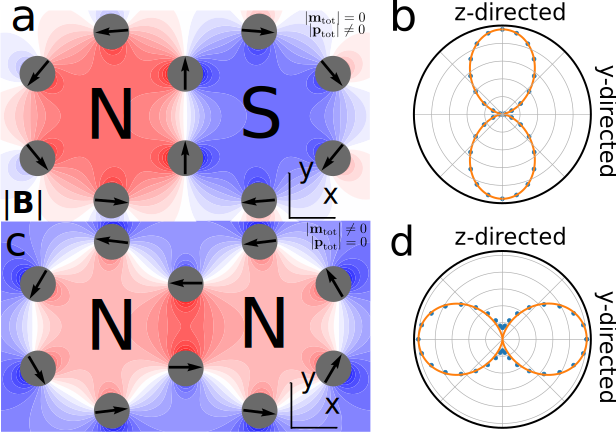
\includegraphics[width=5in]{scattering_patterns.pdf}
\caption{Magnetic field distributions of a magnetic dipole mode (a) and an electric dipole mode (c) in the xy-plane with corresponding radiation patterns (b and d) in the yz-plane. The magnetic dipole exhibits the expected dipolar doughnut, or two lobe, shape with a node along the z-axis. The electric dipole moment also shows the expected pattern with a node along the y-axis.}
\label{scattering}
\end{figure}

Using the scattering patterns in Figure~\ref{scattering} computed from Equation~\ref{dp_dipoles_2}, we can make predictions about how to observe each individual magnetic plasmon resonance. The aN modes support a z-oriented magnetic dipole and radiate in the xy-plane. The NS mode in the 2mer is oriented in the y-direction, and so it radaites in the xz-plane. The cyclic 3mer is more complicated. Due to its threefold symmetry, its x- and y-oriented NS modes are degenerate and linearly dependent, meaning that they can be mutually excited. When exciting the 3mer with a y-oriented electric field, it radiates strongly in the xz-plane and weakly in the yz-plane. Using an x-oriented electric field results in the opposite. When choosing field polarizations that excite both the all-North mode and the North-South mode, the systems radiate very strongly in the direction of light propagation, and exhibit very weak back scattering. Strong forward to backward scattering ratios are also predicted and demonstrated in metal-semiconductor core-shell nanoparticles, which similarly exploit the interference between an electric plasmon and a magnetic plasmon\cite{Kivshar2012}. With these radiative properties in mind, we can now observe each magnetic plasmon separately. By collecting photons in the directions that each plasmon radiates weakly, we should be able to see one more strongly than the other. To help this selectivity, we will preferentially excite each magnetic plasmon using an electron beam.

\section{Angle-Resolved Cathodoluminescence for Observing Spectral Switching}
Electron beam spectroscopies, such as EELS and CL, in a STEM are useful for high spatial and spectral resolution studies of nanomaterials\cite{Coenen2011,CoPol2011,Abajo2013,Polman2014,ARPC}. While EELS measures the probability that a passing electron loses energy to a material, CL measures the probability that an excitation in the sample decays into photon emission. Recent studies have demonstrated the utility of angle-resolved CL spectroscopy to characterize a material. Using a STEM fitted with a parabolic mirror over the sample, the user can collect emitted light with angular information within $0 \leq \theta \leq \pi/2$ and $0 \leq \phi \leq \pi$\cite{Coenen2011,CoPol2011,Polman2014}. Here we show that with the selection rules imposed by the location of the electron beam and the specific directionality of the emission from each magnetic mode, the magnetic modes and their crossing can be observed in spectra. The previous section built up intuition regarding the directionality of light scattered by the magnetic modes of the 2mer and 3mer. This intuition informas the specific angles at which to collect CL spectra. Using the selection rules imposed by the electron beam and the directionality of light, it is possible to distinguish the magnetic modes and observe them switch spectral order.

\begin{figure}
\includegraphics[width=6in]{CL_2mer_3mer.pdf}
\caption{Angle-resolved cathodoluminescence spectra of the 2mer (a and b) and 3mer (c and d). By choosing the beam positions marked on the diagrams and choosing different angles at which to measure the light emitted, the magnetic modes of each oligomer can be disentangled. The colored "x's" correspond to colored traces. The blue traces show a collection angle of $\phi = 3\pi/2$ and the orange traces are for $\phi = \pi$, while both have $\theta = \pi/4$. Simulating these CL experiments with $r_0 = 15$ nm shows the aN modes lower in energy than the NS modes, as predicted. WIth $r_0 = 30$ nm, the modes switch, again as predicted.}
\label{CL_2mer_3mer}
\end{figure}

In Figure~\ref{CL_2mer_3mer} we show point CL spectra on the 2mer and 3mer, with the electron beam positions represented in the diagrams by a blue x and  an orange x chosen to excite the aN modes and the NS modes, respectively. However, due to the symmetry of the model systems, the blue position can weakly excite the NS mode, meaning that signatures of it will appear in both spectra. Recalling that the aN mode should radiate in the xy-plane and the North-South mode should radiate in the z-direction and either the x- or the y- direction, it is possible to distinguish the modes by collecting photons at different angular distributions. The angles chosen are reported in Figure~\ref{CL_2mer_3mer}. These spectra confirm the predictions made in Figure~\ref{scaling}, specifically that between $r_0 = 15$ nm and $r_0 = 30$ nm, the aN mode and the NS mode switch spectral order.

We have now shown that the fully retarded coupled dipole approximation can qualitatively and, to small error, quantitatively predict the eigenenergies and spectral switching of magnetic plasmons, we are prepared to explore more complicated geometries that are active areas of research. Before moving on, we must make a quick note about accuracy. We have chosen Drude model parameters for silver that accurately predict the single plasmon frequency at all the sizes we explore, specifically $\varepsilon_{\infty} = 3.77$, $\hbar\omega_p = 9.15$ eV, and $\hbar\gamma = 0.05$ eV. However, these parameters also appear in the static polarizability which dresses the coupling terms. As a result, any error introduced from the choice of Drude model would increase with increasing particle number. Though this is the case for larger and more complicated systems, we assert that the fully retarded coupled dipole method is qualitatively sound and that magnetic plasmon mode switching is a physical phenomenon.

\section{Eigenspectra and CL Spectra of Hexagonally-Packed Arrays}

In order to show that this discussion of mode-switching is experimentally relevant, we use the intuition we have built from the model systems and previous simulated CL experiments to investigate magnetic oligomer systems of recent interest. Specifically, we look at hexagonally packed clusters of 13, 19, and 31 MNPs originally designed and characterized by Greybush \textit{et al}\cite{Engheta2017}. The arrangement of MNPs and the magnetic plasmon modes that we discuss are shown in Figure~\ref{kagan_fields}. Using the discussion of model systems above as a template, for each system we track the eigenenergies of an aN mode and a NS mode and also show that their switching can be observed in simulated angle-resolved CL measurements.

\begin{figure}
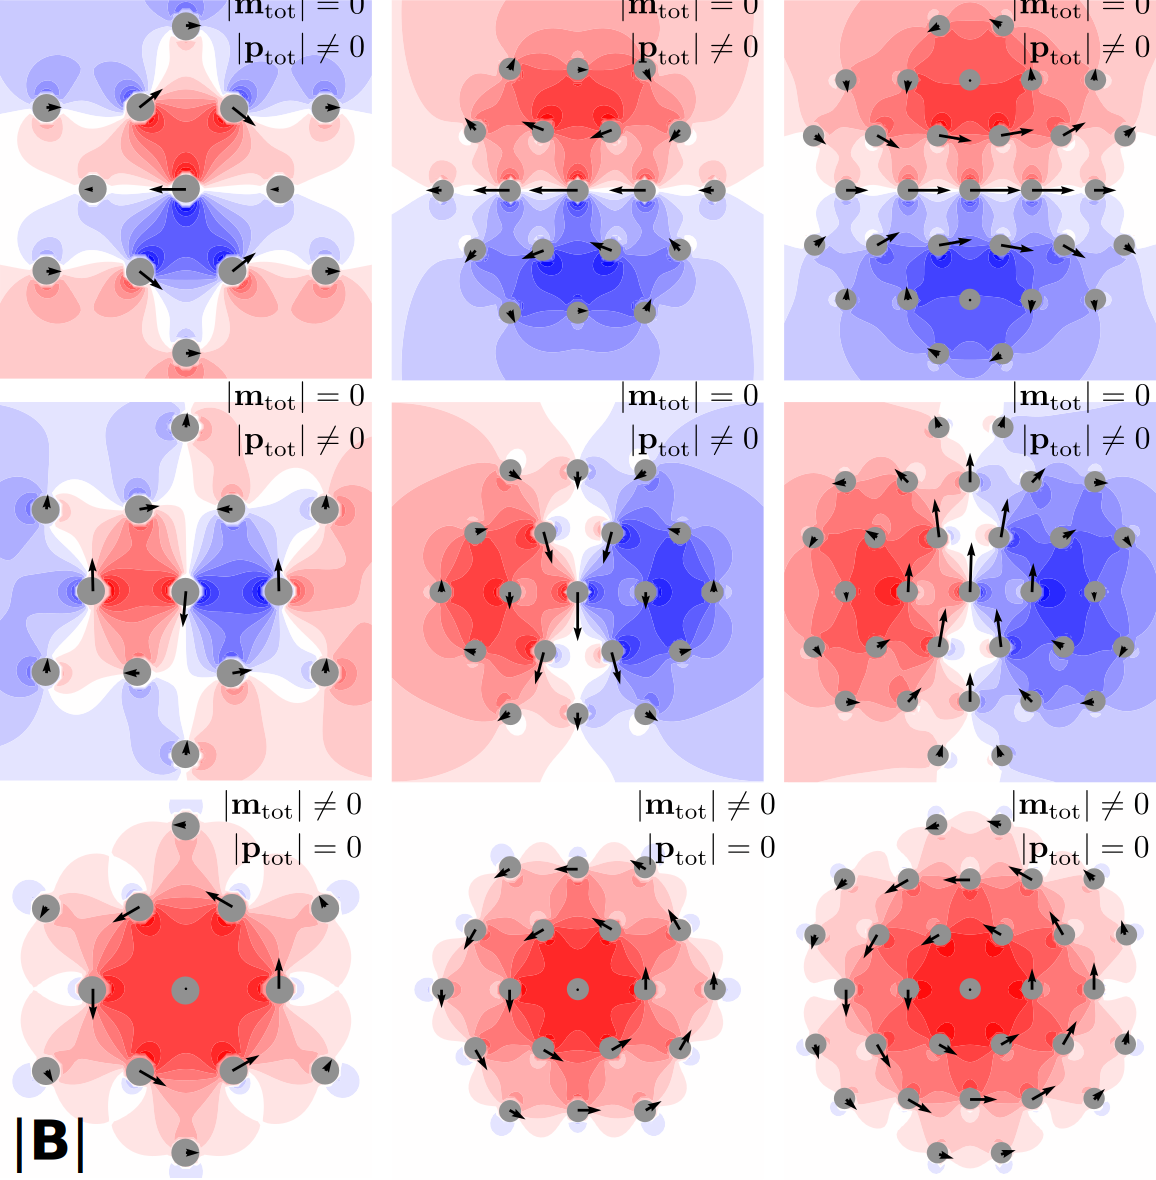
\includegraphics[width=6in]{kagan_fields.pdf}
\caption{Signed magnetic field magnitudes of the modes of the 13-particle (a, b, and c), 19-particle (d, e, and f), and 31-particle (g, h, and i) clusters. Similarly to the 2mer and 3mer from before, we present only those magnetic modes with either NS and electric dipole character (a, b, d, e, g, and h) or with aN and magnetic dipole character (c, f, and i).}
\label{kagan_fields}
\end{figure}

The magnetic modes of the structures shown in Figure~\ref{kagan_fields} show two kinds of magnetic character. The aN mode of each cluster consists of concentric rings of head-to-tail electric dipoles, with a z-oriented magnetic dipole. The NS modes of each cluster, which are degenerate, exhibit two equal-sized regions of out-of-phase magnetic character, as well as net electric dipoles. In fact, the NS modes of these planar arrays behave the same way as the NS modes of the 3mer in that due to the sixfold symmetry, the "x-oriented" and "y-oriented" dipoles are linearly dependent and mutually excitable by a single plane wave. However, because an electron beam excitation would break this symmetry, the two modes can be distinguished between beam positions and angular distributions of radiation.

\begin{figure}
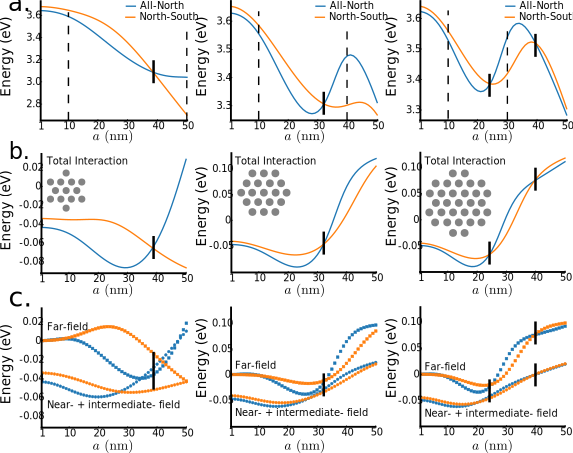
\includegraphics[width=6in]{13_19_31_eigen.pdf}
\caption{Eigenenergies and interaction energies for the magnetic modes of the 13- (a and b), 19- (c and d), and 31-particle (e and f) clusters. Unlike the previous 2mer and 3mer, at very small values of $r_0$, the aN modes are lower in energy than the NS modes. However, for each system a crossing point does occur between $r_0 = 30$ nm and $r_0 = 40$ nm. While the modes of the 13-particle system behave as expected, the aN and NS modes of the larger clusters behave contrary to the intuition built from the earlier model systems. At larger sizes, instead of a monotonic decrease in eigenenergies, the modes exhibit an increase in energy. Looking at the interaction energies, it becomes clear that this is again due to retardation effects, as the term that contributes the most anti-bonding character to the total interaction energy is the far-field. Furthemore, the 31-particle system exhibits a second crossing, unlike the other two structures, and the increase in its eigenenergies is maximized at smaller sizes.}
\label{kagan_eigen}
\end{figure}

The magnetic mode eigenenergies shown in Figure~\ref{kagan_eigen} behave counter to the intuition we have built using the fused, empty ring systems like the 2mer and 3mer. This is because, quite simply, these clusters are constructed from a different aggregation scheme. Though the eigenmodes don't exhibit identical behavior to those shown in Figure~\ref{scaling}, the tools presented earlier are still valid for explaining why the modes cross. Most surprising is the tendency of the modes of the 19- and 31-particle systems to increase in energy at large scale values. This is contrary to the model systems and to plasmonic intuition, in which increasing size causes redshifts. However, we again show the interaction energies, and the dominance of the far-field term is solely responsible for the net positive coupling. In other words, at certain sizes and distances, these magnetic modes become antibonding. This is not so unexpected; separating a MNP dimer causes its resonance frequency to oscillate about a central frequency, from bonding to antibonding and back\cite{vonPlessen2007}. Angle-resolved CL spectra will show that this phenomenon is indeed physical.

\begin{figure}
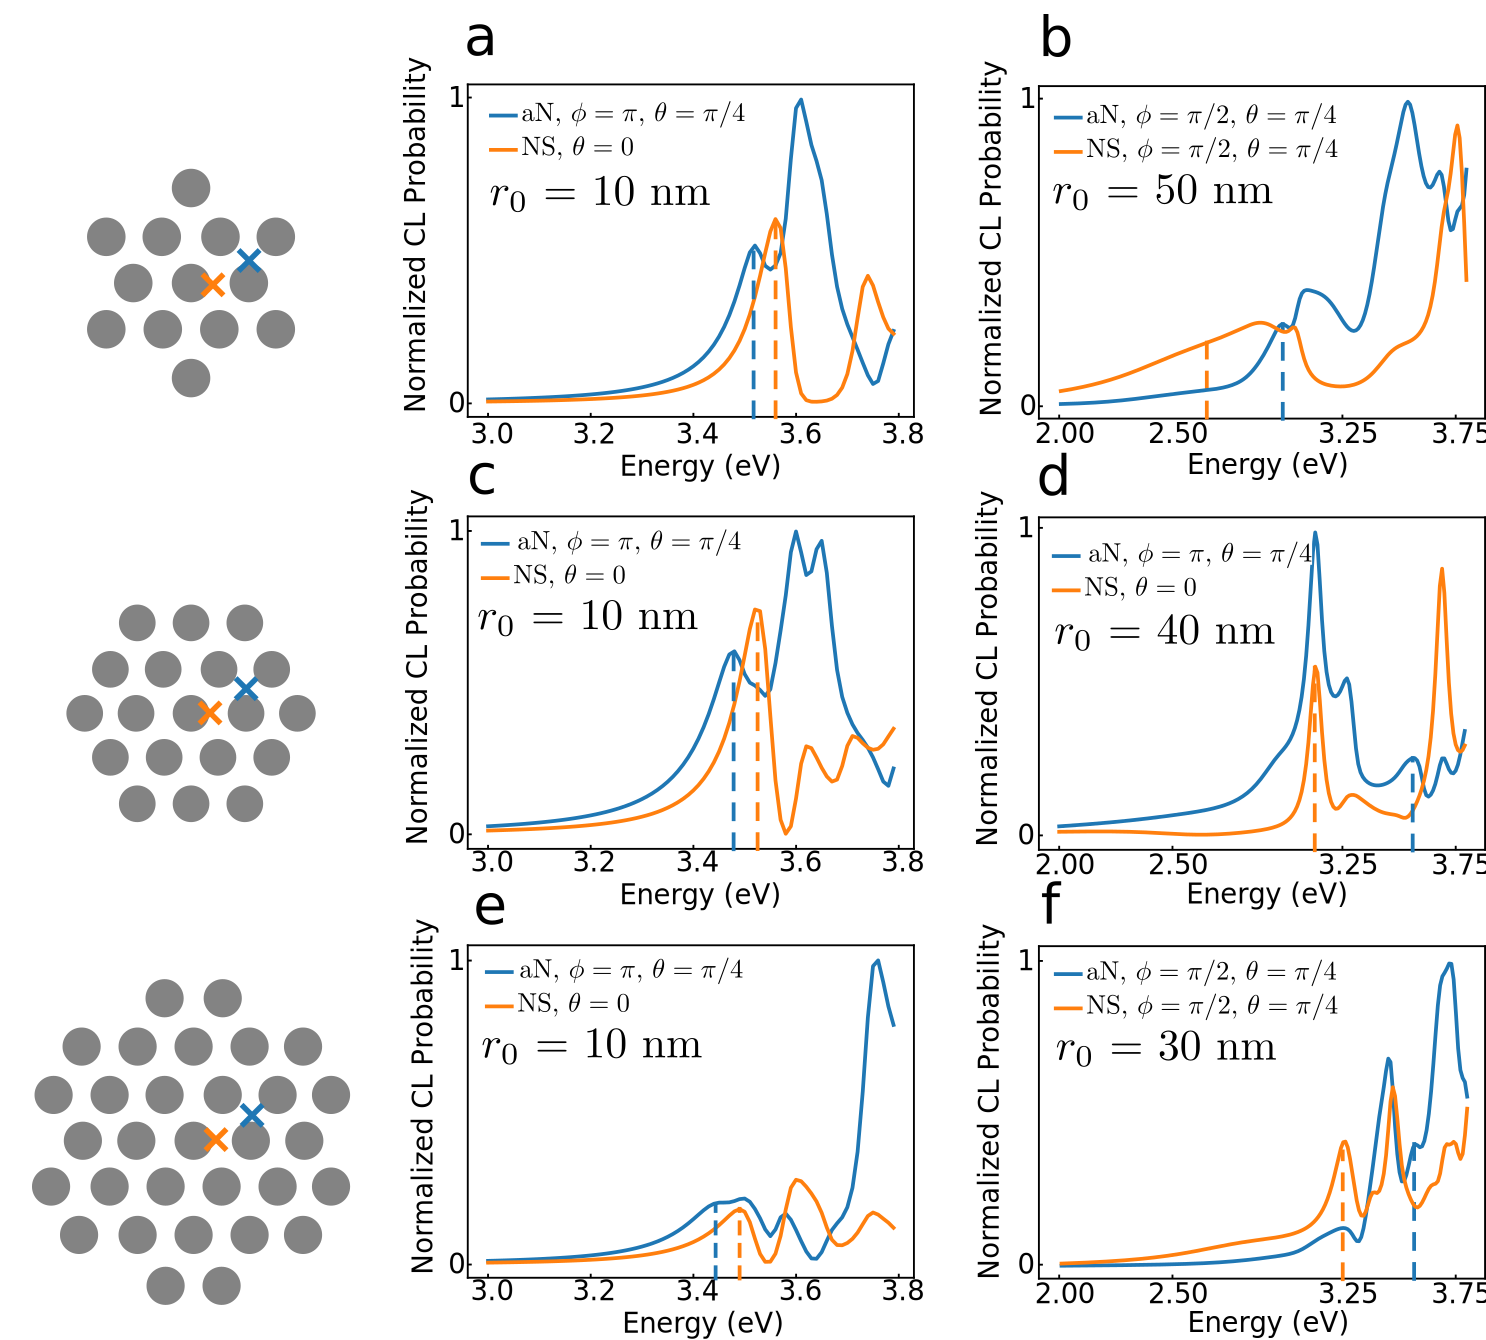
\includegraphics[width=6in]{kagan_CL_spectra.pdf}
\caption{Simulated angle-resolved cathodoluminescence spectra of the 13-, 19-, and 31-particle systems. Blue spectra were acquired at the beam positions marked with a blue x in order to preferentially excite the aN mode. Orange spectra were collected at the points marked with an orange x in order to preferentially excite the x-polarized NS mode. Spectra for the 13-particle aggregate were computed for $r_0 = 10$ nm (a) and $r_0 = 50$ nm (b). Spectra for the 19-particle aggregate were computed for $r_0 = 10$ nm (c) and $r_0 = 40$ nm (d). Spectra for the 31-particle aggregate were computed for $r_0 = 10$ nm (e) and $r_0 = 30$ nm (f). The dashed lines in each spectrum indicate the peak location of the aN modes (blue curves) and the NS modes (orange curves). Each panel also displays the collection angles for each spectrum.}
\label{kagan_CL}
\end{figure}

Figure~\ref{kagan_CL} shows simulated CL spectra for the 13-, 19-, and 31-particle system. The selection rules and radiative properties of each mode help to deconvolute the spectra. Because the aN mode radiates strongly in the xy-plane, and weakly in the z-direction, it is the most easily detected at angles of $theta$ larger than 0 radians. The NS mode can be detected either with $theta$ very close to 0 radians, or in the y-direction for this particular beam position. The aN beam position also weakly excites the NS modes, so the spectrum at that position should exhibit a feature that corroborates the spectral location of that mode. After comparing and contrasting between multiple angular spectra,  we show only those spectra that clearly display shoulders or peaks corresponding to the NS mode or the aN mode.

This analysis is experimentally accessible and can be further supported by computing EELS or CL maps of these clusters. Using the field and dipole plots in Figure~\ref{kagan_fields}, the EELS and CL maps of the aN mode and NS mode should be distinguishable. The aN map will exhibit low probability around the central particle, where the dipole moment is smallest, while the NS mode will exhibit large probability around the central dipole where the dipole moment is largest. As a result, electron beam spectroscopies are the perfect tool to experimentally probe the spectral ordering of magnetic plasmon resonances.

\section{Methods}
Here we show how to derive the equations of motion, and solve an example system of two coupled oscillators. The Hamiltonian for a system of $N$ coupled oscillators

\begin{equation}
H = \sum_{i}\frac{\textbf{p}_i^2}{2m_{\textrm{sp}}}+\frac{1}{2}m_{\textrm{sp}}\omega_{\textrm{sp}}^2\textbf{q}_i^2 - \frac{e}{2}\sum_{j\neq i}\textbf{q}_i\cdot\textbf{E}_j(\textbf{r}_i),
\label{hammy}
\end{equation}

\noindent where $\textbf{p}_i$ are the momenta of the plasmon oscillators with coordinates $\textbf{q}_i$, $m_{\textrm{sp}}$ is the plasmon mass, $\omega_{\textrm{sp}}$ is the plasmon frequency, and $\textbf{E}_j(\textbf{r}_i)$ is defined in Equation~\ref{electric_field_lambda}. The next step is to write Hamilton's equations of motion,

\begin{equation}
\dot{\textbf{p}}_i = -\frac{\partial H}{\partial\textbf{q}_i} = -m_{\textrm{sp}}\omega_{\textrm{sp}}^2\textbf{q}_i + e\sum_{j\neq i}\textbf{E}_j(\textbf{r}_i)
\label{p_dot}
\end{equation}

\noindent and

\begin{equation}
\dot{\textbf{q}}_i = \frac{\partial H}{\partial\textbf{p}_i} = \frac{\textbf{p}_i}{m_{\textrm{sp}}}.
\label{q_dot}
\end{equation}

Finally, taking another time derivative of Equation~\ref{q_dot} and plugging in Equation~\ref{p_dot}, we obtain the equation of motion

\begin{equation}
\ddot{\textbf{q}}_i = -\omega_{\textrm{sp}}^2\textbf{q}_i + \frac{e}{m_{\textrm{sp}}}\sum_{j\neq i}\textbf{E}_j(\textbf{r}_i)
\label{equation_of_motion_again}
\end{equation}

\noindent which is exactly Equation~\ref{equation_of_motion}. From here, introducing time-dependence as a complex exponential, rewriting the electric field in terms of the plasmon coordinate, and performing a Fourier transform results in equations of motion in the frequency domain

\begin{equation}
(\omega_{\textrm{sp}}^2-\omega^2)\textbf{q}_i -\frac{e^2}{m_\textrm{sp}}\sum_{j\neq i}\boldsymbol{\Lambda}_{ij}\cdot\textbf{q}_j = 0.
\label{fourier_eom}
\end{equation}

It is this system of equations for the plasmon oscillator coordinates that we solve for the normal modes. As an example, we demonstrate this calculation for two coupled oscillators displaced and oriented along the x-axis. Knowing the dipole orientation allows us to project out the vector components and reduce the coupling term to a constant, resulting in

\begin{equation}
(\omega_{\textrm{sp}}^2-\omega^2)q_1 -g_{1,2}q_2 = 0
\label{fourier_eom_1}
\end{equation}

and

\begin{equation}
(\omega_{\textrm{sp}}^2-\omega^2)q_2 -g_{1,2}q_1 = 0.
\label{fourier_eom_2}
\end{equation}

Putting these equations of motion in matrix form allows us to solve for the eigenvalues and eigenvectors as follows.

\begin{equation}
\begin{bmatrix}
(\omega_{\textrm{sp}}^2-\omega^2) & -g_{1,2}\\
-g_{1,2} & (\omega_{\textrm{sp}}^2-\omega^2)
\end{bmatrix}
\begin{bmatrix}
q_1\\
q_2
\end{bmatrix}
=
\begin{bmatrix}
0\\
0
\end{bmatrix}
\label{eom_matrix}
\end{equation}

Finding the determinant of this matrix yields the eigenvalues of the collective modes,

\begin{equation}
\omega_{\pm} = \sqrt{\omega_{sp}^2 \pm g_{1,2}}.
\label{eigenvalues}
\end{equation}

\noindent Of course, the coupling terms $g_{1,2}$ in fact depend on the frequency of the collective mode, which is demonstrated in Equation~\ref{electric_field_lambda}. Because of this, the eigenvalue problem must be solved iteratively until the eigenvalues converge. This example can be extended to systems of an arbitrary number of dipoles, and this exact method is used to solve for the eigenvalues of the magnetic plasmon modes.

\section{Conclusion}
Magnetic plasmon oligomers of experimentally relevant size cannot be properly modeled using the quasistatic approximation. We have shown that a fully retarded coupled dipole method accurately predicts the energetics and ordering of magnetic plasmon resonances. Angle resolved cathodoluminescence spectroscopy confirms the predictions of the model, both on fused-ring oligomers and hexagonally-packed clusters of MNPs. This suggests yet another knob to turn in the field of plasmonics: the spectral ordering of resonances. The tunability of the relative phase of magnetic fields will allow advances in information processing, biological detection, and nanoscale etching.


\begin{acknowledgement}
CEI for money, HPC/Hyak/Mox for computing time, Niket and Harrison for good conversations.
\end{acknowledgement}

%%%%%%%%%%%%%%%%%%%%%%%%%%%%%%%%%%%%%%%%%%%%%%%%%%%%%%%%%%%%%%%%%%%%%
%% The appropriate \bibliography command should be placed here.
%% Notice that the class file automatically sets \bibliographystyle
%% and also names the section correctly.
%%%%%%%%%%%%%%%%%%%%%%%%%%%%%%%%%%%%%%%%%%%%%%%%%%%%%%%%%%%%%%%%%%%%%
\bibliography{references}
\end{document}


%While good for theoretical studies of system properties, scale is not tunable in real time, meaning these properties can't be easily measured. Recent research has focused heavily on finding controllable and reversible ways to manipulate the aggregation scheme of a metal nanoparticle array using tools like DNA, polymers, and stretchable embedding media\cite{Yang2016,Ginger2017,NaLiu2017,DanLuo2009}. We employ this idea by fixing the particle radii and the aggregation scheme of the structure and inflating the interparticle distances. Figure~\ref{scaling}e-h shows the results of fixing $r_0$ at 15 and 30 nm and increasing $s$. Increasing the distance between particles regardless of particle size and environment weakens the coupling as the distance approaches infinity, which can be seen in Equation~\ref{electric_field_lambda}. As a result, the collective frequencies of the magnetic modes approach the single plasmon frequency. On the way, the modes oscillate about each other, exhibiting multiple crossings. The amplitude of these crossings appears to increase with increasing particle size and with increasing background dielectric constant, which can be seen in Figure~\ref{scaling}f and h. The quasistatic approximation cannot explain this phenomenon. The fully retarded electric field contains a complex exponential term that depends on interparticle separation. It is this term that dresses all of the interaction terms in the field and changes the sign of the interaction from negative to positive at certain distances. This is clear evidence that the magnetic modes of the 2-mer are tunable in real time in a laboratory with splittings as small as 0.01 eV and as large as 0.1 eV. 

%When two or more metal nanoparticles (MNPs) are brought together, their individual electric plasmons can hybridize to produce new, collective plasmon resonances\cite{Lucas1976,ARAVIND1981,Xu1995,Mischenko1995}. Arranging three or more MNPs on the vertices of a polygon generates a collective mode that resembles a fictitious current loop and produces a sizeable magetic moment in the center of the polygon\cite{Alu2006,Alu2008,Liu2011,Nord2006,Cherqui2014}. These aggregates can couple to and enhance the magnetic field of light, leading to applications such as solar cell enhancement\cite{Graydon2011,Alu2014solar,Le2015solar}, biosensing and detection\cite{Zia2010trans,Noginova2008trans,Wang:13,Fan2015,Wei2015,Shvets2012,Altug2012bio,Nord2011fano}, and information storage and propagation\cite{Zhang2006,NordHal2011,NordHal2012}.

%Of recent interest has been the ability of magnetic plasmons, much like electric plasmons, to hybridize\cite{Cherqui2016}. Similar to how a pair of electric plasmons can produce an electrically bright and an electrically dark mode, a pair of magnetic plasmons can produce a magnetically bright mode and a magnetically dark mode. This understanding opens up new routes to preferentially exciting magnetic and electric plasmons and distinguishing between the different plasmonic modes of a particular aggregate. Studies of the properties of magnetic plasmons have focused on plasmon propagation and hybridization, but have not sought to determine under what circumstances the magnetic plasmons of a system dominate its optical properties. Key to answering this question is the influence of retardation effects.


%This work utilizes and augments a previously published tight-binding model\cite{Cherqui2014}. The model in question maps the electric plasmon of each nanoparticle onto a harmonic oscillator and allows them to couple through quasistatic, near-field interactions using the Hamiltonian


%\begin{equation}
%\frac{H}{\hbar\omega_{\textrm{sp}}} = \frac{1}{2}\sum_{i}\left[\boldsymbol{\Pi}_{i}^2 + \textbf{Q}_{i}^{2}\right] - \frac{\alpha_{\textrm{sp}}}{2}\sum_{i\neq j}\textbf{Q}_{i}\cdot\boldsymbol{\Lambda}_{ij}\cdot\textbf{Q}_{j}.
%\label{full_hammy}
%\end{equation}

%Here, $\omega_{\textrm{sp}}$ is the resonant frequency of the individual electric plasmons, the $\boldsymbol{\Pi}_{i}$ are the generalized momenta conjugate to the generalized coordinates $\textbf{Q}_{i}$, $\alpha_{\textrm{sp}}$ is the polarizability of each individual MNP, and $\boldsymbol{\Lambda}_{ij}$ is the near-field dipole-dipole relay tensor. In this work, retardation effects are incorporated into the dipole-dipole relay tensor through the intermediate- and far-field terms in the dipole electric field as follows:

%\begin{equation}
%\boldsymbol{\Lambda}_{ij} = \left[\left(\frac{1}{r_{ij}^3} - \frac{\textrm{i}\omega}{cr_{ij}^2}\right)\left(3\hat{\textbf{n}}_{ij}\hat{\textbf{n}}_{ij} - \textbf{1}\right) + \frac{\omega^2}{c^2r_{ij}}\left(\textbf{1} - \hat{\textbf{n}}_{ij}\hat{\textbf{n}}_{ij}\right)\right]e^{\textrm{i}\omega/c r},
%\label{dipoledipole}
%\end{equation}

%where $r_{ij}$ is the distance between the $i^{\textrm{th}}$ and $j^{\textrm{th}}$ dipoles along the unit vector $\hat{\textbf{n}}_{ij}$, \textbf{1} is the unit dyad, $c$ is the speed of light, and $\omega$ is the collective frequency at which all of the dipoles oscillate. Using Equations~\ref{full_hammy} and ~\ref{dipoledipole}, Hamilton's equations of motion,

%\begin{equation}
%\ddot{\textbf{Q}}_{i} = -\textbf{Q}_{i} + \sum_{j\neq i}\boldsymbol{Lambda}_{ij}\cdot\textbf{Q}_{j}
%\label{eom}
%\end{equation}

% can be found and the system of equations can be solved for the eigenvalues and eigenvectors of the nanoparticle array. The eigenvectors are the generalized coordinates corresponding to each dipole moment in the aggregate. It is important to note that because the eigenvalues, the collective frequencies, appear in the coupling terms, this will result in a system of transcendental equations which must be solved iteratively. 

%In this paper, three model systems are considered. Following previous work, the model systems are constructed from fused, six-member rings of silver nanospheres, resembling conjugated hydrocarbon rings. The aggregates considered are a two-ring system, a linear three-ring system, and a triangular three-ring system. Solving for the magnetic eigenmodes of each system results in a set of eigenvectors for each mode which correspond to electric dipole moments. Figure~\ref{field_plots} shows the oligomers, the dipole moments on each sphere, and the magnetic field distribution computed from\cite{jackson_classical_1999}

%\begin{equation}
%\textbf{B}_{\textrm{tot}}(\textbf{r},\omega) = \frac{\omega^2}{c^2}\sum_{j}(\hat{\textbf{n}}_{j}\times\textbf{p}_{j})\frac{e^{\textrm{i}\omega/c r_j}}{r_j}\left(1 - \frac{c}{\textrm{i}\omega r_{j}}\right).
%\label{magnetic_field}
%\end{equation}

